\chapter{Experiments and User Experience Evaluation}

Proper quality assurance leads to a better user experience, however, by quantifying user experience, we can try to understand better and improve it. This chapter will focus on experiments that are measuring the performance of the Tribler core, with a particular focus on user experience. Various common operations executed by users in Tribler are identified, discussed and measured.

\section{Experiments environment}
The experiments with the Tribler core are performed on a virtual private server. We tried to keep close to the specifications of a machine that an actual user could be using. The virtual server has 8GB of memory and 1 processor with 4 cores (with a clock speed of 2,5GHz). The used operation system is Ubuntu 15.10.\\\\
If not stated otherwise, the default values of the Tribler configuration file are used. These default values can be found in the `defaults.py` file in the source code directory of Tribler\footnote{https://github.com/Tribler/tribler/blob/devel/Tribler/Core/defaults.py}.

\section{Start-up experience}
The very first interaction that users are making with Tribler, is the process of starting. During the boot process, several operations are performed:
\begin{itemize}
	\item The connection to the sqlite database is opened. If this database does not exist, it will be created.
	\item Dispersy is started and the enabled communities are loaded.
	\item Various Tribler components are loaded and initialized, including the video streaming server, the REST API, the remote torrent handler and the leveldb store.
\end{itemize}
To measure the average start-up time, Tribler is started 30 times. In half of the runs, Tribler is started for the first time, with no prior existing state directory. In the other half of the runs, a database with just over 100.000 torrents is used. This database is the result of running Tribler idle for several hours. Also, a filled Dispersy database is used for the second half of the runs. In both scenarios, there are no active downloads. The experiment starts when the \emph{start} method of the \emph{Session} object is called and ends when the notification that Tribler has started, is observed. The results are displayed in Figure \ref{fig:startup_experiment}.\\\\
It is clear that that size of the database has impact on the time for Tribler to completely boot. However, this impact is relatively minor since Tribler still starts within a second. In both plots, we see some outliers.

\begin{figure}[!h]
	\centering
	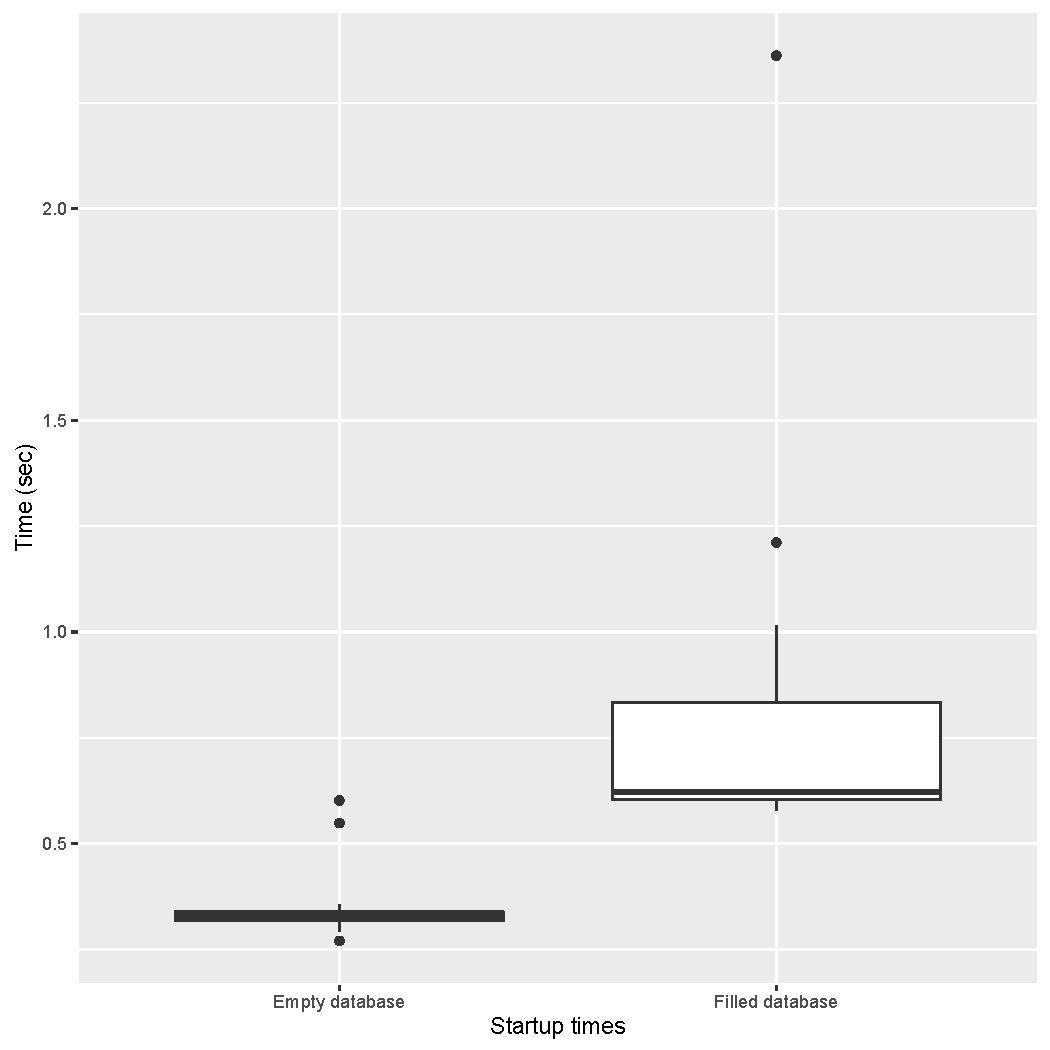
\includegraphics[width=0.6\columnwidth]{images/experiments/startup}
	\caption{Test.}
	\label{fig:startup_experiment}
\end{figure}

\section{Remote keyword search}
...

\section{Local keyword search}
...

\section{First content discovery}
...

\section{Channel subscription}
...

\section{Fetching metainfo of torrents}
...

\section{Video server performance}
...

\section{Performance on low-end devices}
...